\label{4_measure}

\section{Naměřené výsledky a vyhodnocení}

Pro \textbf{měření} na klastru Star jsem vybral tři instance, které mají \textbf{sekvenční} dobu běhu na jednom uzlu Star mezi 2 a 10 minutami -- jedná se o mnou vygenerované instance 27\_19, 28\_19 a 28\_24. Pro měření jsem upravil zdrojové kódy sekvenčního, OpenMP (datový paralelismus) a MPI programů tak, aby měřily pouze čas výpočtu \textit{(jak dlouho trvá volání příslušné funkce \mintinline{c}{weight})} a zároveň jsem přidal do OpenMP a MPI programu parametr nastavující \textbf{počet} vláken, na kterých se program spustí.

Následně jsem použil předvytvořené skripty z \mintinline{c}{/home/mpi}, které jsem vhodně \textbf{upravil} a umístil do složky \mintinline{c}{scripts}. Nachází se zde tedy \textbf{skripty} pro spuštění sekvenčního programu, OpenMP a MPI programu s 2, 4, 8, 10, 16 a 20 jádry. Dále jsem si vytvořil pomocné skripty pro \textbf{kompilaci} a \textbf{spuštění}:

\begin{listing}[H]
    \begin{minted}{shell}
# Build Sequential solution
g++ -Wall -pedantic main_seq.cpp -O3 -o main_seq

# Build OpenMP solution
g++ -Wall -pedantic -fopenmp main_par_data.cpp -O3 -o main_par

# Build MPI solution
mpic++ main.cpp -O3 -fopenmp -o main_pdp
    \end{minted}
    \caption{Skript pro kompilaci na Staru}
\end{listing}

\begin{listing}[H]
    \begin{minted}{shell}
# Start sequential job
qrun 20c 1 pdp_serial scripts/serial_job.sh

for i in {2,4,8,10,16,20}
do
  # Start OpenMP jobs
  qrun 20c 1 pdp_serial "scripts/openmp_job$i.sh"

  # Start MPI jobs (master + 2 slaves)
  qrun 20c 3 pdp_long "scripts/parallel_job$i.sh"

  # Start MPI jobs (master + 3 slaves)
  qrun 20c 4 pdp_fast "scripts/parallel_job$i.sh"
done
    \end{minted}
    \caption{Skript pro spuštění na Staru. Všimněte si, že k spuštění na masteru a 2 slavech používám frontu \mintinline{c}{pdp_long}, protože zvláště na nižším počtu jader zde hrozí, že by program nestihl doběhnout pod 3 minuty.}
\end{listing}

Skript jsem \textbf{spustil} na každé z těchto instancí a výsledky jsem zapsal do následující \textbf{tabulky} a vytvořil z nich následující grafy (upozornění: osa y používá logaritmickou škálu), které budu analyzovat v kapitole \nameref{5_end}:

\begin{table}[H]
    \centering
    \begin{tabular}{l|r|r|r}
    Graf                    & 27\_19    & 28\_19    & 28\_24    \\
    \hline
    Váha                    & 15 470    & 15 758    & 18 729    \\
    Rekurzivních volání     & 21.3 G    & 38.7 G    & 65.5 G    \\
    \hline
    Čas (sekvenční)         & 166.583 s & 321.817 s & 530.419 s \\
    \hline
    Čas (OMP, 2 vlákna)     &  82.231 s & 158.141 s & 260.696 s \\
    Čas (OMP, 4 vlákna)     &  96.659 s &  80.066 s & 291.926 s \\
    Čas (OMP, 8 vláken)     &  20.707 s & 122.108 s &  65.995 s \\
    Čas (OMP, 10 vláken)    &  20.801 s &  79.593 s &  98.695 s \\
    Čas (OMP, 16 vláken)    &  10.583 s &  20.267 s &  98.644 s \\
    Čas (OMP, 20 vláken)    &  14.709 s &  20.239 s &  65.750 s \\
    \hline
    Čas (MPI/3, 2 vlákna)   &  47.160 s &  97.083 s & 128.017 s \\
    Čas (MPI/3, 4 vlákna)   &  20.385 s &  39.226 s & 142.958 s \\
    Čas (MPI/3, 8 vláken)   &  29.564 s &  43.320 s &  32.337 s \\
    Čas (MPI/3, 10 vláken)  &  20.321 s &  33.892 s &  48.161 s \\
    Čas (MPI/3, 16 vláken)  &   5.255 s &  19.590 s &  48.055 s \\
    Čas (MPI/3, 20 vláken)  &   7.479 s &  17.185 s &  32.178 s \\
    \hline
    Čas (MPI/4, 2 vlákna)   &  35.114 s &  58.276 s &  95.822 s \\
    Čas (MPI/4, 4 vlákna)   &  15.251 s &  29.345 s & 106.708 s \\
    Čas (MPI/4, 8 vláken)   &  22.264 s &  38.630 s &  24.295 s \\
    Čas (MPI/4, 10 vláken)  &  14.984 s &  29.035 s &  36.120 s \\
    Čas (MPI/4, 16 vláken)  &   3.923 s &   7.572 s &  35.722 s \\
    Čas (MPI/4, 20 vláken)  &   5.602 s &  10.785 s &  24.098 s \\
    \end{tabular}
    \caption{Tabulka naměřených časů běhů}
    \label{4_times}
\end{table}

\begin{figure}[H]
    \centering
    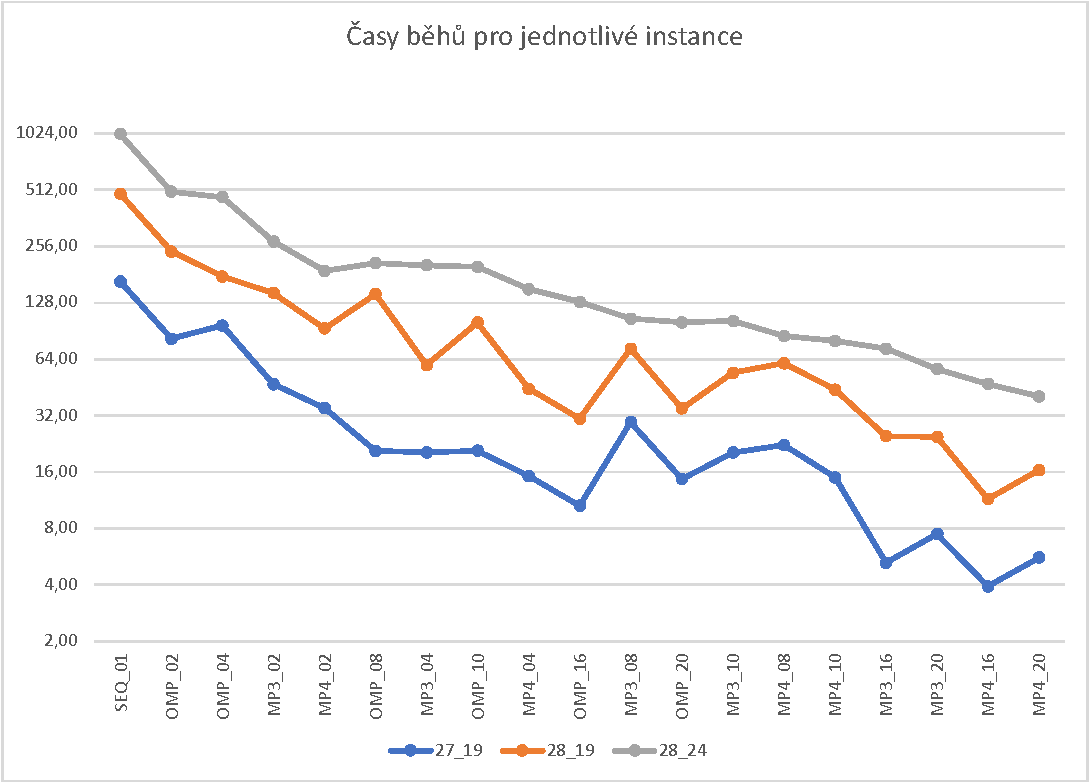
\includegraphics[width=\textwidth]{fig/4_1.pdf}
    \caption{Časy běhu na jednotlivých instancích}
    \label{4_timesgraph}
\end{figure}

\begin{figure}[H]
    \centering
    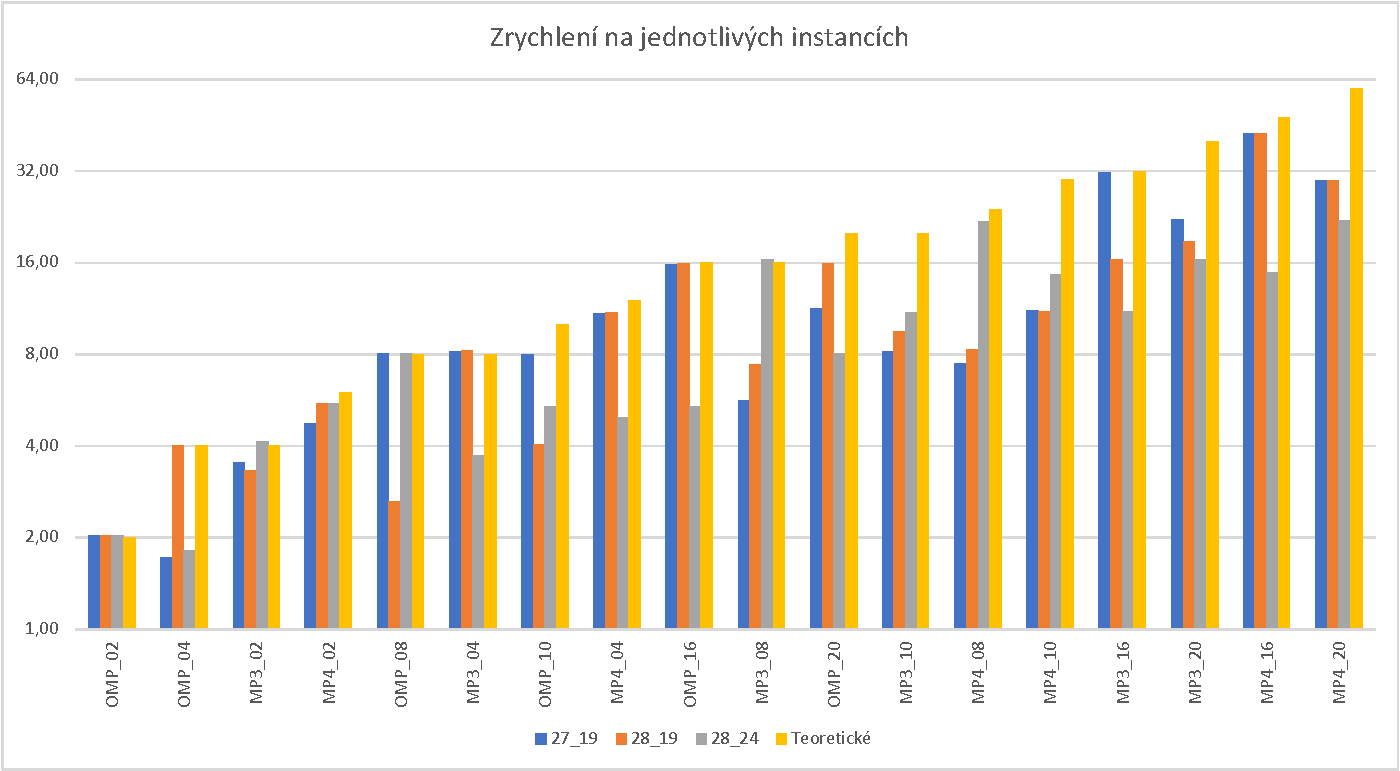
\includegraphics[width=\textwidth]{fig/4_2.pdf}
    \caption{Zrychlení na jednotlivých instancích}
    \label{4_speedup}
\end{figure}
